\documentclass[UTF8]{ctexart}
\usepackage{algorithm}
\usepackage{algorithmic}
\usepackage{amsmath,amssymb}
\usepackage{booktabs}
\usepackage{geometry}
\usepackage{tikz}

\renewcommand{\algorithmicrequire}{ \textbf{Input:}} %Use Input in the format of Algorithm
\renewcommand{\algorithmicensure}{ \textbf{Output:}} %UseOutput in the format of Algorithm

\geometry{a4paper,scale=0.7}

\begin{document}
SA22225226 李青航
~\\
\noindent\textbf{164}

\textbf{i. }

$\{x_4,x_1,x_0\}$用二进制表示为00010011,下一个为00010100,
所以下一个组合为$\{x_4,x_2\}$

\textbf{ii. }

同理$\{x_7,x_5,x_3\}$10101000,下一个为10101001$\{x_7,x_5,x_3,x_0\}$

\textbf{iii. }

$\{x_7,x_6,x_5,x_4,x_3,x_2,x_1,x_0\}$11111111,最后一个了

\textbf{iv. }

$\{x_0\}$00000001,下一个00000010$\{x_1\}$

~\\
\noindent\textbf{172}

\textbf{i. }010100110

$\sigma(010100110)=4$是偶数,改变取反$a_0$,得010100111

\textbf{ii. }110001100

$\sigma(110001100)=4$是偶数,改变取反$a_0$,得110001101

\textbf{iii. }111111111

$\sigma(111111111)=9$,最右一位1的$a_j$为$j=$lowbit$(111111111)=0$位,所以将$a_{j+1}$
位取反,为111111101

~\\
\noindent\textbf{192}

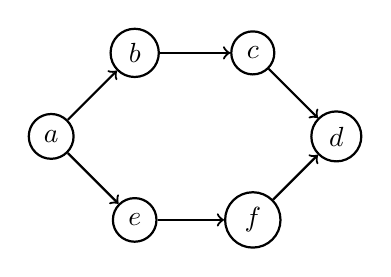
\begin{tikzpicture}[node distance={15mm}, thick, main/.style = {draw, circle}] 
\node[main] (1) {$a$}; 
\node[main] (2) [above right of=1] {$b$}; 
\node[main] (3) [below right of=1] {$e$}; 
\node[main] (4) [right of=2] {$c$}; 
\node[main] (5) [right of=3] {$f$}; 
\node[main] (6) [below right of=4] {$d$};
\draw[->] (1) -- (2); 
\draw[->] (1) -- (3); 
\draw[->] (2) -- (4); 
\draw[->] (3) -- (5); 
\draw[->] (4) -- (6);
\draw[->] (5) -- (6);
\end{tikzpicture} 

如Hasse图所示(横着的),显然,就是一个覆盖关系。

所有偏序集关系,有$abecfd, abefcd, aebcfd, aebfcd, abcefd, aefbcd.$

~\\
\noindent\textbf{207}

由于图5-1,第8行是 1    ,   8    ,   28   ,   56    ,  70   ,   56   ,   28   ,   8   ,    1
由帕斯卡公式得

第9行  1  ,     9    ,   36  ,    84   ,   126  ,   126   ,  84  ,    36  ,    9    ,   1

第10行 1       ,10     , 45      ,120   ,  210    , 252  ,   210  ,   120   ,  45 ,     10   ,   1

~\\
\noindent\textbf{220}

由$k{n\choose k}=n{n-1 \choose k-1}$和二项式定理中设$x=1,y=-1$的交错和等于0得

\begin{equation}
    \nonumber
    \begin{aligned}
        0
&={n\choose 1}-2{n\choose 2}+3{n\choose 3}+\dots+(-1)^{n-1}
n{n\choose n}\\
&=(n-1){n-1\choose 0}-(n-1){n-1\choose 1}+(n-1){n-1\choose 2}+\dots
+(-1)^{n-1}(n-1){n-1\choose n-1}\\
&=(n-1)\left[{n-1\choose 0}-{n-1\choose 1}+{n-1\choose 2}+\dots
+(-1)^{n-1}{n-1\choose n-1}\right]\\
&=(n-1)\cdot 0\\
&=0
    \end{aligned}
\end{equation}
得证

~\\
\noindent\textbf{228}

\textbf{i. }$$24\choose 10$$

\textbf{ii. }

两步,先到朋友家,再到学校,乘法原理
$${9\choose 4}\cdot {15\choose 6}$$

\textbf{iii. }

三步
$$
{\dbinom{9}{4}} \cdot {\dbinom{9}{3}} \cdot {\dbinom{6}{3}} 
$$

\textbf{iv. }

就是\textbf{ii. }的结果减去\textbf{iii. }的结果

~\\
\noindent\textbf{235}

因为
$$
(1+x)^{n}=\sum ^{n}_{k=0} {n\choose k}x^k
$$

又有
$$
(1+x)^{m_1}(1+x)^{m_2}(1+x)^{m_3}=(1+x)^{m_1+m_2+m_3}
$$

对于上式,展开两边,$x^n$的系数相同

左边$x^n$系数就是题目原式
$$
\sum_{r,s,t\ge 0, r+s+t=n}{m_1\choose r}{m_2\choose s}
{m_3\choose t}
$$

右边的$x_n$系数就是
$$
{m_1+m_2+m_3\choose n}
$$

所以,左右$x_n$系数相等
$$
\sum_{r,s,t\ge 0, r+s+t=n}{m_1\choose r}{m_2\choose s}
{m_3\choose t}
=
{m_1+m_2+m_3\choose n}
$$



\end{document}

